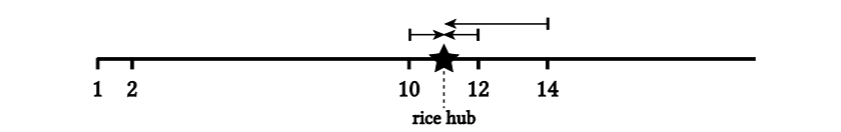
\includegraphics[width=18cm]{ricehub.png}

В этом примере существует несколько оптимальных местоположений рисохранилища. Можно поместить его в любой точке с целыми координатами от $10$ до $14$ включительно. На рисунке выше показано одно из этих оптимальных местоположений. В этом случае можно перевезти рис от полей в точках с координатами $10$, $12$ и $14$ до рисохранилища. Для каждого из этих оптимальных расположений общая стоимость транспортировки будет не более $6$ бат. Очевидно, что никакое из возможных расположений рисохранилища не позволит собирать рис более чем с трёх полей, таким образом, это решение оптимально и процедура \t{besthub} должна возвращать число $3$.